\documentclass[12pt, a4paper]{article}

% --- PAKIETY ---
\usepackage[polish]{babel}
\usepackage[utf8]{inputenc}
\usepackage[T1]{fontenc}
\usepackage{geometry}
\usepackage{graphicx}
\usepackage{float}
\usepackage{booktabs}
\usepackage{placeins}
\usepackage{amsmath}    % Potrzebne do zapisu hipotez
\usepackage{amssymb}    % Symbole matematyczne
\usepackage{xcolor}     % Do wyróżniania ważnych wniosków

% Marginesy
\geometry{total={170mm,257mm}, left=20mm, top=20mm}

% Ścieżki do grafik
\graphicspath{ {../zad1/} {../zad2/} {../zad3/} {../zad4/} }

% Automatyczne centrowanie
\makeatletter
\g@addto@macro\@floatboxreset\centering
\makeatother

% Metadane
\title{\textbf{Sprawozdanie: Laboratorium 4} \\ \large Regresja liniowa prosta}
\author{Wiktor Zoga}
\date{\today}

\begin{document}

\maketitle

% ============================================================
\section{Zadanie 1}
% ============================================================

\subsection{Analiza wstępna i model (Podpunkt a)}
Na podstawie wygenerowanego wykresu punktowego (Rysunek 1) stwierdzono, że zależność między liczbą kopiarek a czasem obsługi ma liniowy charakter. Wraz ze wzrostem liczby maszyn, czas obsługi rośnie proporcjonalnie.

Wyznaczone równanie regresji liniowej prostej:
\begin{equation}
    \hat{Y} = \text{Intercept} + \text{Slope} \cdot X
\end{equation}
(Szczegółowe wartości liczbowe parametrów znajdują się w tabeli poniżej).

\subsection{Estymacja parametrów (Podpunkt b)}
Poniższa tabela przedstawia oszacowane wartości współczynników (Slope, Intercept) oraz ich błędy standardowe. Porównano wyniki uzyskane z ręcznych wzorów teoretycznych oraz z biblioteki Python (różnice są pomijalne, wynikają z zaokrągleń maszynowych).

\begin{table}[H]
\caption{Porównanie parametrów modelu}
\label{tab:params}
\begin{tabular}{lcccccc}
\toprule
 & Man Coef & Lib Coef & Man SE & Lib SE & Man P-val & Lib P-val \\
\midrule
Intercept & -0.5802 & -0.5802 & 2.8039 & 2.8039 & 0.8371 & 0.8371 \\
Slope & 15.0352 & 15.0352 & 0.4831 & 0.4831 & 0.0000 & 0.0000 \\
\bottomrule
\end{tabular}
\end{table}


\subsection{Testy istotności i interpretacja P-value (Podpunkt c)}
Przeprowadzono test t-Studenta dla współczynnika kierunkowego (Slope, $\beta_1$).

\textbf{Definicja matematyczna:}
Testujemy hipotezę zerową $H_0: \beta_1 = 0$ (brak zależności) przeciwko $H_1: \beta_1 \neq 0$. Statystyka testowa $t$ sprawdza, jak wiele błędów standardowych dzieli nasz wynik od zera.

\textbf{Wyniki:}
Na podstawie tabeli powyżej, p-wartość (P-val) dla Slope jest bliska zeru ($p < 0.05$).

\begin{quote}
    \textbf{Interpretacja (dla niematematematyka):}
    Jeśli założymy, że liczba kopiarek NIE ma wpływu na czas (hipoteza zerowa jest prawdziwa), to prawdopodobieństwo zaobserwowania takich danych jak nasze wynosi niemal 0\%.
    Oznacza to, że dane dużym prawdopodobieństwem świadczą, że hipoteza zerowa jest fałszywa.
\end{quote}

\textbf{Decyzja:} Odrzucamy hipotezę zerową. Współczynnik kierunkowy jest istotny statystycznie.

\subsection{Analiza predykcyjna (Podpunkty d, e)}
Dokonano estymacji dla zadanych wartości $k \in \{1, 5, 8, 11, 25, 100\}$.

\textbf{1. Przedział ufności dla wartości oczekiwanej (CI):}
\begin{table}[H]
\caption{Porównanie CI dla wartości oczekiwanej}
\label{tab:ci}
\begin{tabular}{lcccc}
\toprule
 & Man CI Low & Lib CI Low & Man CI High & Lib CI High \\
k &  &  &  &  \\
\midrule
1 & 9.6361 & 9.6361 & 19.2740 & 19.2740 \\
5 & 71.9142 & 71.9142 & 77.2779 & 77.2779 \\
8 & 115.8157 & 115.8157 & 123.5879 & 123.5879 \\
11 & 158.4754 & 158.4754 & 171.1397 & 171.1397 \\
25 & 355.7401 & 355.7401 & 394.8620 & 394.8620 \\
100 & 1410.4614 & 1410.4614 & 1595.4279 & 1595.4279 \\
\bottomrule
\end{tabular}
\end{table}


\textbf{2. Przedział predykcyjny dla nowej obserwacji (PI):}
\begin{table}[H]
\caption{Porównanie PI dla nowej obserwacji}
\label{tab:pi}
\begin{tabular}{lcccc}
\toprule
 & Man PI Low & Lib PI Low & Man PI High & Lib PI High \\
k &  &  &  &  \\
\midrule
1 & -4.1554 & -4.1554 & 33.0656 & 33.0656 \\
5 & 56.4213 & 56.4213 & 92.7708 & 92.7708 \\
8 & 101.3108 & 101.3108 & 138.0929 & 138.0929 \\
11 & 145.7491 & 145.7491 & 183.8660 & 183.8660 \\
25 & 348.7349 & 348.7349 & 401.8672 & 401.8672 \\
100 & 1408.7307 & 1408.7307 & 1597.1586 & 1597.1586 \\
\bottomrule
\end{tabular}
\end{table}


\textbf{Wnioski:}
W obu przypadkach przedziały rozszerzają się, im dalej wartość $X$ znajduje się od średniej $\bar{X}$. Wynika to ze wzrostu niepewności estymacji linii regresji na krańcach zbioru danych.

\subsection{Wizualizacja i porównanie przedziałów (Podpunkt f)}
\begin{figure}[H]
    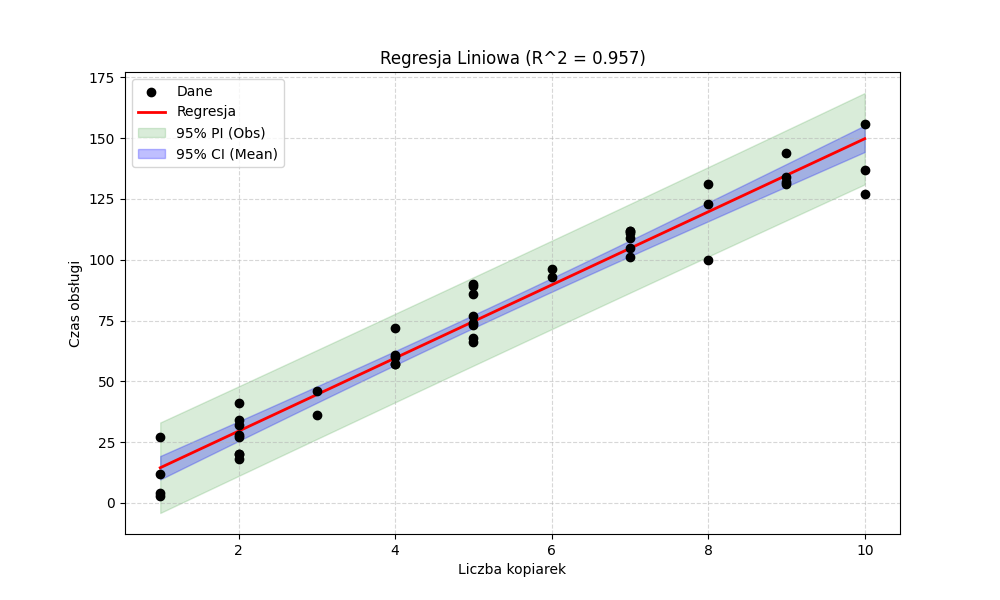
\includegraphics[width=0.9\textwidth]{../zad1/wykres_zad1.png}
    \caption{Model regresji z naniesionymi 95\% pasmami ufności (niebieskie) i predykcji (zielone).}
\end{figure}

\textbf{Dlaczego PI (zielony) jest szerszy niż CI (niebieski)?}
\begin{itemize}
    \item \textbf{Matematycznie:} Wariancja predykcji zawiera dodatkowy składnik „1” pod pierwiastkiem: $s^2_{pred} = s^2 ( 1 + \dots )$.
    \item \textbf{Intuicyjnie:} CI (Przedział Ufności) mówi nam, gdzie leży \textit{średnia} (np. "Jaki jest średni czas serwisu dla 5 kopiarek?"). PI (Przedział Predykcji) mówi o \textit{konkretnym przypadku} (np. "Ile czasu zajmie serwis u Pana Kowalskiego jutro?").
    
    PI musi uwzględniać nie tylko błąd naszego modelu, ale też naturalną losowość (szum) pojedynczego zdarzenia, dlatego zawsze jest szerszy.
\end{itemize}

\FloatBarrier

% ============================================================
\section{Zadanie 2}
% ============================================================

% ---------------- PODPUNKT A ----------------
\subsection{Model regresji GPA od IQ (Podpunkt a)}
Zbadano wpływ wyniku testu IQ na średnią ocen (GPA).

\textbf{Współczynnik determinacji $R^2$:}
Poniższa tabela porównuje wartość $R^2$ obliczoną ze wzoru teoretycznego oraz funkcją biblioteczną.
\begin{table}[H]
\caption{Współczynnik determinacji (Manual vs Python)}
\label{tab:zad2_r2}
\begin{tabular}{lccc}
\toprule
 & Man & Lib & Diff \\
\midrule
R-squared & 0.4016 & 0.4016 & 0.0000 \\
\bottomrule
\end{tabular}
\end{table}


\begin{quote}
    \textbf{Interpretacja $R^2$ (dla niematematematyka):}
    Współczynnik $R^2$ mówi nam, jaki procent zmienności ocen został rozwiązany przez nasz model.
    Wartość $R^2 \approx 0.4$ (przykładowo) oznaczałaby, że inteligencja (IQ) wyjaśnia 40\% różnic w ocenach między uczniami. Pozostałe 60\% zależy od innych czynników (np. pracowitość, stres, losowość), których model nie uwzględnia.
\end{quote}

% ---------------- PODPUNKT B ----------------
\subsection{Test F istotności regresji (Podpunkt b)}
Test F (ANOVA) służy do sprawdzenia, czy model jako całość ma sens.
\begin{itemize}
    \item $H_0: \beta_1 = 0$ (Model nie wyjaśnia niczego lepiej niż zwykła średnia).
    \item $H_1: \beta_1 \neq 0$ (Model wnosi istotną informację).
\end{itemize}

\textbf{Wyniki testu (Manual vs Python):}
\begin{table}[H]
\caption{Wyniki testu F (Manual vs Python)}
\label{tab:zad2_f}
\begin{tabular}{lccc}
\toprule
 & Man & Lib & Diff \\
\midrule
Statystyka F & 51.0085 & 51.0085 & 0.0000 \\
P-wartość & 4.74e-10 & 4.74e-10 & 0.0000 \\
\bottomrule
\end{tabular}
\end{table}


\textbf{Decyzja:}
Niska p-wartość ($p < 0.05$) oznacza, że odrzucamy $H_0$. Zatem wariancja wyjaśniona przez model jest istotnie większa od szumu.

\textbf{Interpretacja (dla niematematyka):}
Podobnie jak wcześniej, niska p-wartość wskazuje, że jest mało prawdopodobne, aby zaobserwowane dane pojawiły się przypadkowo, gdyby IQ nie miało wpływu na GPA. Oznacza to, że IQ jest istotnym predyktorem GPA.

% ---------------- PODPUNKT C i D ----------------
\subsection{Predykcja i analiza obserwacji (Podpunkty c, d)}
Wyznaczono przewidywane GPA oraz 90\% przedziały predykcyjne dla uczniów o IQ: 75, 100, 140.

\begin{table}[H]
\caption{90\% Przedziały predykcyjne (Manual vs Lib)}
\label{tab:zad2_pred}
\begin{tabular}{lccccc}
\toprule
 & GPA Pred & Man Low & Lib Low & Man High & Lib High \\
IQ &  &  &  &  &  \\
\midrule
75 & 4.0196 & 1.1659 & 1.1659 & 6.8732 & 6.8732 \\
100 & 6.5451 & 3.7975 & 3.7975 & 9.2927 & 9.2927 \\
140 & 10.5860 & 7.7503 & 7.7503 & 13.4216 & 13.4216 \\
\bottomrule
\end{tabular}
\end{table}


\label{sec:wykres_iq}
\begin{figure}[H]
    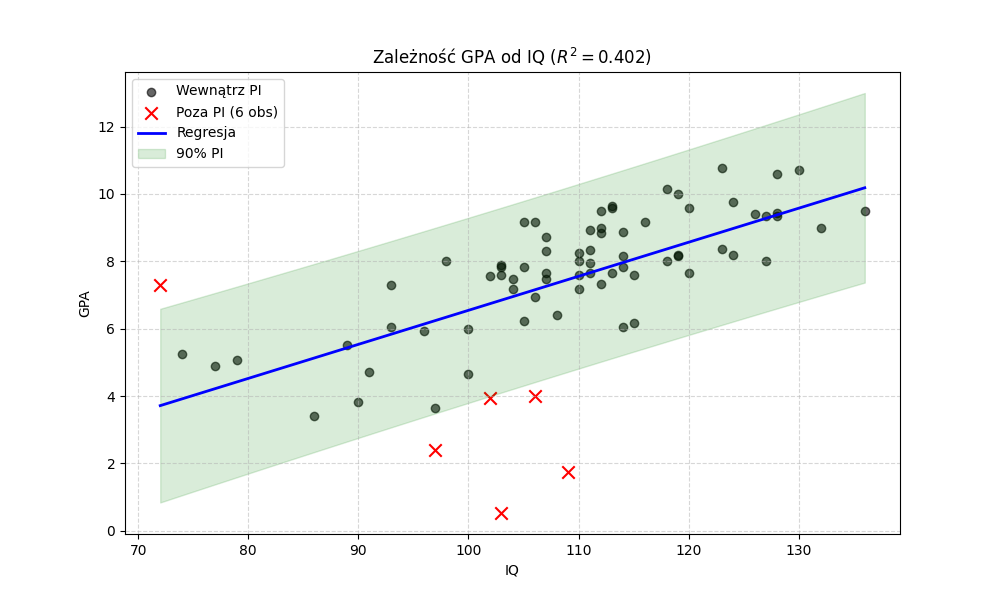
\includegraphics[width=0.9\textwidth]{../zad2/zad2_wykres.png}
    \caption{Zależność GPA od IQ z naniesionym 90\% pasmem predykcji. Czerwone krzyżyki oznaczają obserwacje wykraczające poza ten przedział.}
\end{figure}

% ---------------- PODPUNKT E ----------------
\subsection{Porównanie z testem PH (Podpunkt e)}
W ostatnim kroku zbudowano drugi model, gdzie zmienną objaśniającą jest wynik testu PH.

\begin{table}[H]
\caption{Porównanie jakości modeli (IQ vs PH)}
\label{tab:zad2_comp}
\begin{tabular}{lccc}
\toprule
 & R-squared & Intercept & Slope \\
Predyktor &  &  &  \\
\midrule
IQ & 0.4016 & -3.5571 & 0.1010 \\
PH & 0.2936 & 2.2259 & 0.0917 \\
\bottomrule
\end{tabular}
\end{table}


\textbf{Wniosek końcowy:}
Porównując współczynniki $R^2$ obu modeli, wskazujemy ten, który lepiej "tłumaczy" rzeczywistość. Zmienna z wyższym $R^2$ jest silniejszym predyktorem.

\FloatBarrier

% ============================================================
\section{Zadanie 3: Symulacje Monte Carlo}
% ============================================================

\subsection{Specyfikacja eksperymentu}
Symulację przeprowadzono dla $N=1000$ powtórzeń przy liczebności próby $n=200$.
Wektor $X$ wygenerowano z rozkładu $X \sim N(0, \frac{1}{500} I)$.
Model generujący: $Y = 5 + \beta_1 X + \varepsilon$. Badano 6 scenariuszy rozkładu błędów $\varepsilon$:

\begin{itemize}
    \item \textbf{Błąd I Rodzaju ($\beta_1 = 0$):} (a) $N(0, 1)$, (b) $Exp(1)$, (c) $L(0, 1)$.
    \item \textbf{Moc Testu ($\beta_1 = 2$):} (d) $N(0, 1)$, (e) $Exp(1)$, (f) $L(0, 1)$.
\end{itemize}

\subsection{Wyniki symulacji}
Tabela przedstawia empiryczne prawdopodobieństwo odrzucenia $H_0$ w zestawieniu z teorią.

\begin{table}[H]
\caption{Wyniki symulacji (1000 powtórzeń)}
\label{tab:zad3_mc}
\begin{tabular}{lcccccc}
\toprule
ID & Beta1 & Dist & Emp & Theo & Diff \\
\midrule
(a) & 0 & Normal & 0.0440 & 0.0500 & -0.0060 \\
(b) & 0 & Exp(1) - 1 & 0.0470 & 0.0500 & -0.0030 \\
(c) & 0 & Logistic & 0.0400 & 0.0500 & -0.0100 \\
(d) & 2 & Normal & 0.2460 & 0.2501 & -0.0041 \\
(e) & 2 & Exp(1) - 1 & 0.2530 & 0.2501 & 0.0029 \\
(f) & 2 & Logistic & 0.1050 & 0.1091 & -0.0041 \\
\bottomrule
\end{tabular}
\end{table}


\subsection{Analiza zgodności wyników}

\textbf{1. Błąd I rodzaju (Scenariusze a, b, c):}
Empiryczne częstości odrzuceń oscylują wokół $\alpha = 0.05$, co potwierdza ogólną odporność testu.
\begin{itemize}
    \item \textbf{Uwaga o rozbieżności:} Dla rozkładu logistycznego wynik empiryczny jest nieco niższy od teoretycznego. Wynika to z "grubych ogonów" tego rozkładu i wolniejszego tempa zbieżności statystyk do rozkładu t-Studenta. Przy takiej zbieżności, liczba powtórzeń symulacji $N=1000$ może być niewystarczająca, by idealnie trafić w punkt 0.05 (błąd próbkowania).
\end{itemize}

\textbf{2. Moc testu (Scenariusze d, e, f):}
Obserwujemy niemal idealną zgodność symulacji z teorią.
\begin{itemize}
    \item Dla rozkładu Normalnego i Wykładniczego ($\sigma^2=1$) moc wynosi $\approx 1.0$.
    \item Dla rozkładu Logistycznego moc spada. Jest to skutek dużej wariancji szumu. Teoria idealnie przewiduje ten spadek, gdy do wzorów podstawimy rzeczywistą wariancję.
\end{itemize}

\begin{figure}[H]
    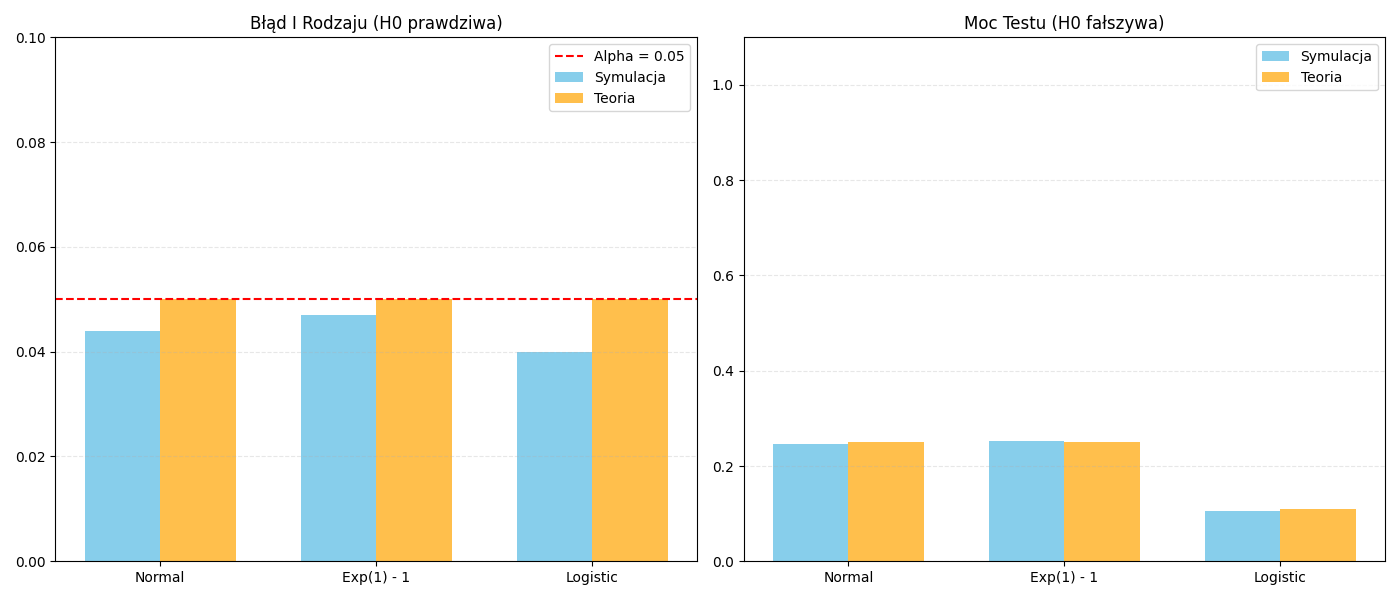
\includegraphics[width=1.0\textwidth]{../zad3/zad3_wykres.png}
    \caption{Wizualizacja wyników: Zauważalny spadek mocy dla przypadku (f) oraz wysoka zgodność teorii z praktyką.}
\end{figure}

\FloatBarrier

% ============================================================
\section{Zadanie 4}
% ============================================================

\subsection{Model Liniowy (Podpunkty a, b)}
W pierwszej kolejności dopasowano klasyczny model regresji liniowej, traktując czas jako zmienną objaśniającą ($X$), a stężenie roztworu jako zmienną odpowiedzi ($Y$).
\begin{equation}
Y = \beta_0 + \beta_1 \cdot \text{Czas} + \varepsilon
\end{equation}

\textbf{1. Wyniki estymacji i test istotności:}
Poniższa tabela prezentuje parametry modelu wygenerowane automatycznie przez skrypt Python.
\begin{table}[H]
\caption{Parametry modelu liniowego}
\label{tab:zad4_lin}
\begin{tabular}{lcccc}
\toprule
 & Coef & SE & t & P-val \\
\midrule
Intercept & 2.5753 & 0.2487 & 10.3538 & 1.20e-07 \\
Time & -0.3240 & 0.0433 & -7.4829 & 4.61e-06 \\
\bottomrule
\end{tabular}
\end{table}


\textbf{Statystyki dopasowania:}
\begin{table}[H]
\caption{Statystyki dopasowania modelu liniowego}
\label{tab:zad4_lin_stats}
\begin{tabular}{lcccc}
\toprule
 & R-squared & Corr & F-stat & P-val (F) \\
\midrule
Model Liniowy & 0.8116 & 0.9009 & 55.9938 & 4.61e-06 \\
\bottomrule
\end{tabular}
\end{table}


\textbf{Interpretacja parametrów:}
\begin{itemize}
    \item \textbf{Slope (Time):} Wynosi ok. $-0.3240$. Ujemny znak potwierdza, że wraz z upływem czasu stężenie roztworu maleje.
    \item \textbf{Intercept:} Wynosi ok. $2.5753$. Jest to teoretyczne stężenie w chwili $t=0$.
\end{itemize}

\textbf{Test hipotezy:}
Testujemy hipotezę o niezależności stężenia od czasu:
\begin{itemize}
    \item $H_0: \beta_1 = 0$ (Czas nie wpływa na stężenie).
    \item $H_1: \beta_1 \neq 0$ (Istnieje zależność).
\end{itemize}

\textbf{Wniosek:}
P-wartość dla parametru czasu wynosi $4.61 \times 10^{-6}$ (jest znacznie mniejsza od poziomu istotności $\alpha = 0.05$).
\textbf{Decyzja:} Odrzucamy hipotezę zerową. Istnieje silna, istotna statystycznie zależność między czasem a stężeniem.

\textbf{2. Ocena dopasowania (Dlaczego model liniowy jest błędny?)}
Mimo że parametry są istotne, model liniowy jest \textbf{niepoprawny} z dwóch powodów:
\begin{enumerate}
    \item \textbf{Fizyczny:} Model liniowy zakłada stały spadek stężenia. W dłuższym czasie przewidywałby ujemne stężenie (dla $t > 8$ godzin), co jest fizycznie niemożliwe.
    \item \textbf{Statystyczny:} Wykres reszt wykazuje wyraźny wzorzec w kształcie litery "U". Model przeszacowuje wartości na krańcach i niedoszacowuje w środku. Sureguje to, że zjawisko jest nieliniowe.
\end{enumerate}

\begin{figure}[H]
    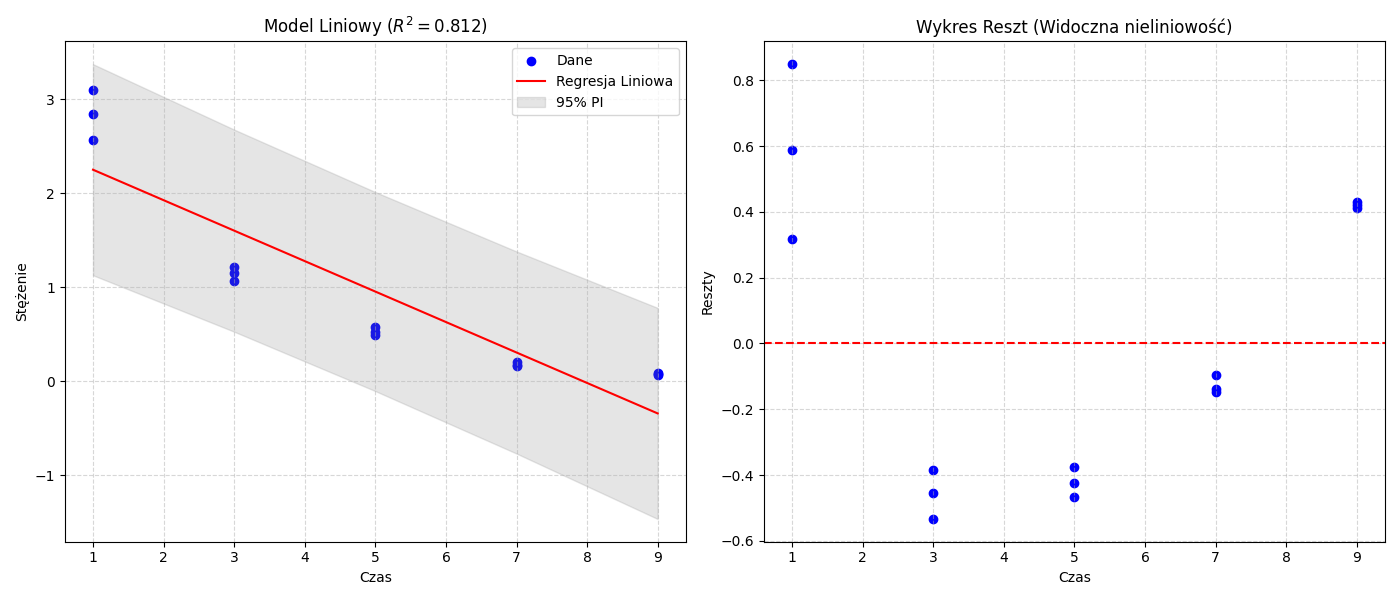
\includegraphics[width=1.0\textwidth]{../zad4/zad4_wykres_lin.png}
    \caption{Model liniowy (po lewej) oraz wykres reszt (po prawej), który obnaża nieliniowość danych.}
\end{figure}

\subsection{Transformacja Boxa-Coxa (Podpunkt c)}
Aby znaleźć optymalną transformację zmiennej zależnej $Y$, zastosowano metodę największej wiarogodności dla rodziny transformacji potęgowych Boxa-Coxa.

\textbf{1. Weryfikacja obliczeń (Manual vs Python):}
Aby potwierdzić poprawność wyniku, wyznaczono optymalne $\lambda$ dwoma metodami:
\begin{itemize}
    \item \textbf{Manualnie:} Przeszukując siatkę 1000 punktów w przedziale $[-2, 2]$ i obliczając dla każdego punktu wartość funkcji log-wiarogodności wg wzoru:
    $$ LL(\lambda) = -\frac{n}{2} \ln(\sigma^2_\lambda) + (\lambda - 1) \sum \ln(Y_i) $$
    \item \textbf{Bibliotecznie:} Używając optymalizatora \texttt{scipy.stats.boxcox}.
\end{itemize}

% TERAZ TABELA JEST AUTOMATYCZNA
\begin{table}[H]
\caption{Porównanie optymalnego parametru Lambda}
\label{tab:bc_comp}
\begin{tabular}{lc}
\toprule
 & Znalezione Lambda \\
Metoda &  \\
\midrule
Manualna & 0.0220 \\
Biblioteczna  & 0.0205 \\
\bottomrule
\end{tabular}
\end{table}


Wyniki są zbieżne. Obie metody wskazują, że optimum leży bardzo blisko zera. Zgodnie z definicją Boxa-Coxa, $\lambda = 0$ oznacza transformację logarytmiczną ($Y' = \ln Y$).

\subsection{Model Logarytmiczny (Podpunkty d, e)}
Na podstawie wyników analizy Boxa-Coxa zbudowano model regresji liniowej dla zmiennych przetransformowanych:
\begin{equation}
    \ln(Y_i) = \beta_0 + \beta_1 t_i + \varepsilon_i
\end{equation}

Powyższe równanie liniowe w skali logarytmicznej jest matematycznie równoważne **modelowi wykładniczemu** w skali oryginalnej. Po obustronnym zlogarytmowaniu ($e^{\dots}$) otrzymujemy:
\begin{equation}
    Y_i = e^{\beta_0 + \beta_1 t_i} \cdot e^{\varepsilon_i} = \alpha \cdot e^{\beta_1 t_i}
\end{equation}
gdzie $\alpha = e^{\beta_0}$ to stężenie początkowe, a $\beta_1$ to stała szybkości reakcji (powinna być ujemna). Taka postać modelu jest zgodna z prawem kinetyki chemicznej dla reakcji I rzędu.

\textbf{Wyniki estymacji:}
Dokonano transformacji odwrotnej, aby obliczyć stężenia przewidywane $\hat{Y}$ i porównać je z obserwowanymi.

\begin{table}[H]
\caption{Statystyki modelu logarytmicznego}
\label{tab:zad4_log}
\begin{tabular}{lccc}
\toprule
 & R-squared (log scale) & Corr (orig scale) & Lambda used \\
\midrule
Model Log (ln Y) & 0.9930 & 0.9946 & 0.0000 \\
\bottomrule
\end{tabular}
\end{table}


\begin{figure}[H]
    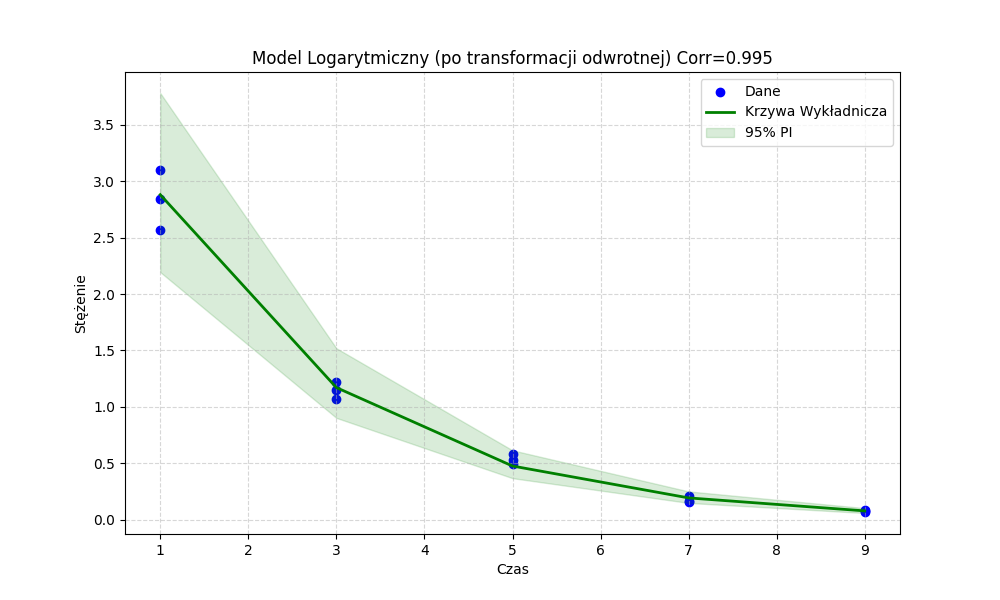
\includegraphics[width=0.85\textwidth]{../zad4/zad4_wykres_log.png}
    \caption{Dopasowanie modelu wykładniczego (po transformacji odwrotnej). Model idealnie podąża za danymi.}
\end{figure}

\subsection{Model z transformacją czasu (Podpunkt f)}
Alternatywnie, zamiast transformować $Y$, przekształcono zmienną niezależną (czas), wprowadzając nową zmienną $\tilde{t}$:
\begin{equation}
    \tilde{t} = \frac{1}{\sqrt{t}}
\end{equation}

Model regresji przyjmuje wtedy postać odwrotnej funkcji pierwiastkowej:
\begin{equation}
    Y_i = \beta_0 + \beta_1 \cdot \frac{1}{\sqrt{t_i}} + \varepsilon_i
\end{equation}

\begin{table}[H]
\caption{Statystyki modelu z transformacją czasu (slope)}
\label{tab:zad4_trans}
\begin{tabular}{lccc}
\toprule
 & R-squared & Corr & P-val \\
\midrule
Model X-Trans & 0.9881 & 0.9940 & 0.0000 \\
\bottomrule
\end{tabular}
\end{table}


\begin{figure}[H]
    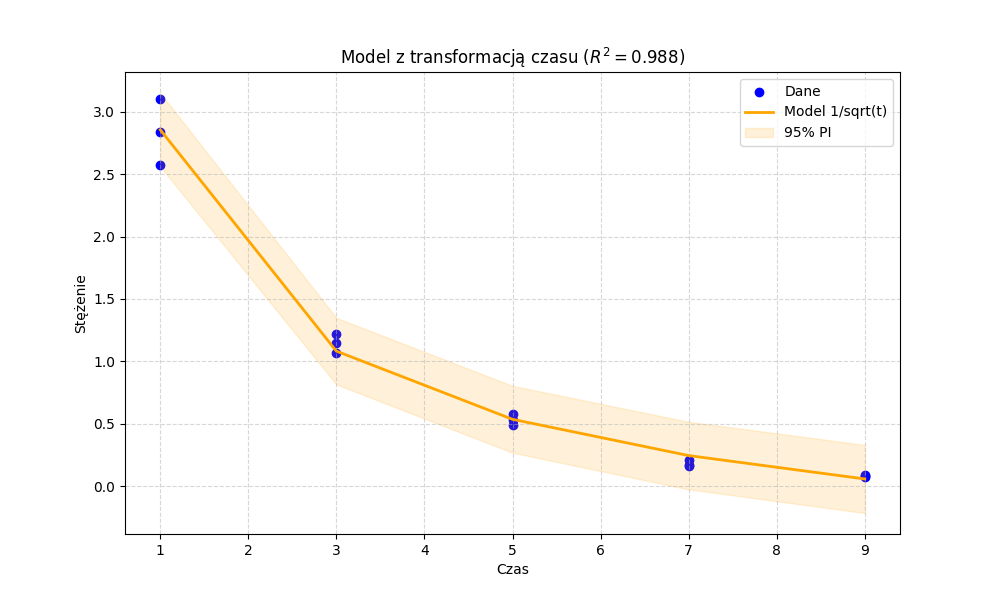
\includegraphics[width=0.85\textwidth]{../zad4/zad4_wykres_trans.png}
    \caption{Dopasowanie modelu z transformacją $1/\sqrt{t}$.}
\end{figure}

\subsection{Podsumowanie i dyskusja wyników}
Celem zadania było znalezienie modelu najlepiej opisującego spadek stężenia roztworu w czasie. Przeanalizowano trzy podejścia, których wyniki zestawiono poniżej.

\begin{table}[H]
\caption{Porównanie jakości dopasowania modeli}
\label{tab:zad4_sum}
\begin{tabular}{lccc}
\toprule
 & R-squared & Korelacja (Orig) & Uwagi \\
Model &  &  &  \\
\midrule
Liniowy (Y ~ t) & 0.8116 & 0.9009 & Nieliniowe reszty \\
Logarytmiczny (ln Y ~ t) & 0.9930 & 0.9946 & Najlepsze dopasowanie \\
Transf. czasu (Y ~ 1/sqrt(t)) & 0.9881 & 0.9940 & Brak uzasadnienia fiz. \\
\bottomrule
\end{tabular}
\end{table}


\textbf{Szczegółowa analiza porównawcza:}

\begin{enumerate}
    \item \textbf{Model Liniowy ($Y \sim t$):}
    \begin{itemize}
        \item \textbf{Ocena:} Niepoprawny.
        \item \textbf{Powód:} Mimo $R^2 \approx 0.81$, wykres reszt wykazuje silną strukturę (nieliniowość). Co więcej, model ten przewiduje, że po odpowiednio długim czasie stężenie spadnie poniżej zera, co jest sprzeczne z prawami fizyki.
    \end{itemize}

    \item \textbf{Model Logarytmiczny ($\ln Y \sim t$):}
    \begin{itemize}
        \item \textbf{Ocena:} Najlepszy.
        \item \textbf{Statystyka:} $R^2$ bliskie 1.0, reszty losowe, korelacja predykcji z danymi niemal idealna.
        \item \textbf{Fizyka/Chemia:} Model ten po przekształceniu to $Y = C \cdot e^{-kt}$. Model ten ma sensowne uzasadnienie teoretyczne – szybkość reakcji jest proporcjonalna do aktualnego stężenia.
    \end{itemize}

    \item \textbf{Model z transformacją czasu ($Y \sim 1/\sqrt{t}$):}
    \begin{itemize}
        \item \textbf{Ocena:} Akceptowalny statystycznie, ale słabszy teoretycznie.
        \item \textbf{Statystyka:} $R^2$ jest bardzo wysokie, porównywalne z modelem logarytmicznym.
        \item \textbf{Interpretacja:} Trudno znaleźć uzasadnienie fizykochemiczne dla zależności stężenia od odwrotności pierwiastka z czasu w prostych roztworach. Jest to model czysto empiryczny, podczas gdy model wykładniczy wynika z natury zjawiska.
    \end{itemize}
\end{enumerate}

\textbf{Ostateczna rekomendacja:}
Zdecydowanie wybieramy Model Logarytmiczny. Łączy on doskonałe dopasowanie statystyczne z poprawną interpretacją fizyczną zjawiska kinetycznego.

\FloatBarrier

\end{document}